% ============================================================
%  Chapter 14 -- Conclusions to Bayesian Machine Learning
%               in Quantitative Finance
%  Bayesian Machine Learning in Quantitative Finance:
%  Theory and Practical Applications (Springer, 2025)
%  Mongwe, Mbuvha & Marwala
%  Beamer slides -- pdflatex compatible
% ============================================================
\documentclass[aspectratio=169,10pt]{beamer}

\usetheme{Madrid}
\usecolortheme{seahorse}
\usefonttheme{professionalfonts}
\setbeamertemplate{footline}[frame number]
\setbeamertemplate{navigation symbols}{}

% ── packages ────────────────────────────────────────────────
\usepackage{amsmath,amssymb,amsfonts}
\usepackage{bm}
\usepackage{graphicx}
\usepackage{booktabs}
\usepackage{listings}
\usepackage{xcolor}
\usepackage{tikz}
\usetikzlibrary{arrows.meta,positioning,shapes.geometric,calc}
\usepackage{array}
\usepackage{hyperref}

\graphicspath{{figures/}}

% ── listings style ──────────────────────────────────────────
\lstset{
  language=Python,
  basicstyle=\ttfamily\scriptsize,
  numbers=left,
  numberstyle=\tiny\color{gray},
  frame=single,
  backgroundcolor=\color{gray!7},
  keywordstyle=\color{blue!80!black}\bfseries,
  commentstyle=\color{green!50!black}\itshape,
  stringstyle=\color{orange!80!black},
  showstringspaces=false,
  tabsize=2,
  breaklines=true,
  breakatwhitespace=true,
  numbersep=6pt,
}

% ── convenience macros ──────────────────────────────────────
\newcommand{\Real}{\mathbb{R}}
\newcommand{\Prob}{\mathbb{P}}
\newcommand{\Ex}{\mathbb{E}}
\newcommand{\thetav}{\theta}
\newcommand{\Data}{\mathcal{D}}

% ── title ───────────────────────────────────────────────────
\title[Bayesian ML in QF -- Ch.14]{Bayesian Machine Learning in Quantitative Finance}
\subtitle{Chapter 14: Conclusions}
\author{Based on Mongwe, Mbuvha \& Marwala}
\date{}

% ============================================================
\begin{document}
% ============================================================

\begin{frame}
  \titlepage
\end{frame}

\begin{frame}{Outline}
  \tableofcontents
\end{frame}

% ============================================================
\section{The Whole Book at a Glance}
% ============================================================

\begin{frame}[allowframebreaks]{Big-Picture Recap: Chapters 3--13, One Table}
  \begin{block}{Intuition}
    Chapter 1 opened with a coin flip and four open questions
    (explainability, parameter uncertainty, principled model selection,
    input relevance). Chapter 2 gave us the computational engines
    (MCMC and variational inference). Every chapter since has been the
    same Bayesian recipe -- prior $\times$ likelihood, normalized by the
    evidence -- applied to a new corner of quantitative finance. Before we
    summarize contributions and future work, here is the whole book on
    one page.
  \end{block}

  \begin{center}
  {\scriptsize
  \begin{tabular}{@{}clll@{}}
    \toprule
    \textbf{Ch.} & \textbf{Application} & \textbf{Bayesian ML method(s)} & \textbf{Theme} \\
    \midrule
    2  & Background: training \& evaluating Bayesian models & Variational inference, MCMC & Background \\
    3  & SABR model calibration (interest-rate skew) & MALA, HMC, Separable Shadow HMC & Derivative modeling \\
    4  & Equity volatility surfaces (SA, Europe) & Single-/multi-output Gaussian processes & Derivative modeling \\
    5  & European option prices (JSE, emerging mkt) & Mixture of normalizing flows & Derivative modeling \\
    6  & Corporate credit ratings & Sparse \& distributed (product-of-experts) GPs & Financial management \\
    7  & Recovery on charged-off loans & Bayesian logistic regr.\ via MALA, HMC, SSHHMC & Financial management \\
    8  & Audit opinion model selection & NF harmonic-mean evidence (MALA/HMC/NUTS) & Financial management \\
    9  & Unauthorized municipal expenditure & BLR-ARD via MH, MALA, HMC, Magnetic HMC & Financial management \\
    10 & Motor insurance claims likelihood & Bayesian neural net + Laplace approx., ARD & Insurance \& investments \\
    11 & Nelson--Siegel yield curve calibration & HMC, Separable Shadow HMC, NUTS & Insurance \& investments \\
    12 & Yield curve model selection & Static \& dynamic nested sampling (evidence) & Insurance \& investments \\
    13 & Bayesian investment analyst (JSE) & BLR-ARD via MCMC (multiple samplers) & Insurance \& investments \\
    \bottomrule
  \end{tabular}
  }
  \end{center}

  \textbf{Notice the pattern:} every row is the same story -- a
  point-estimate machine learning problem, re-cast so that the posterior
  (over parameters, over model choice, or over an entire function) is the
  object of interest. That is the thread this chapter ties together.

  \framebreak

  \begin{center}
    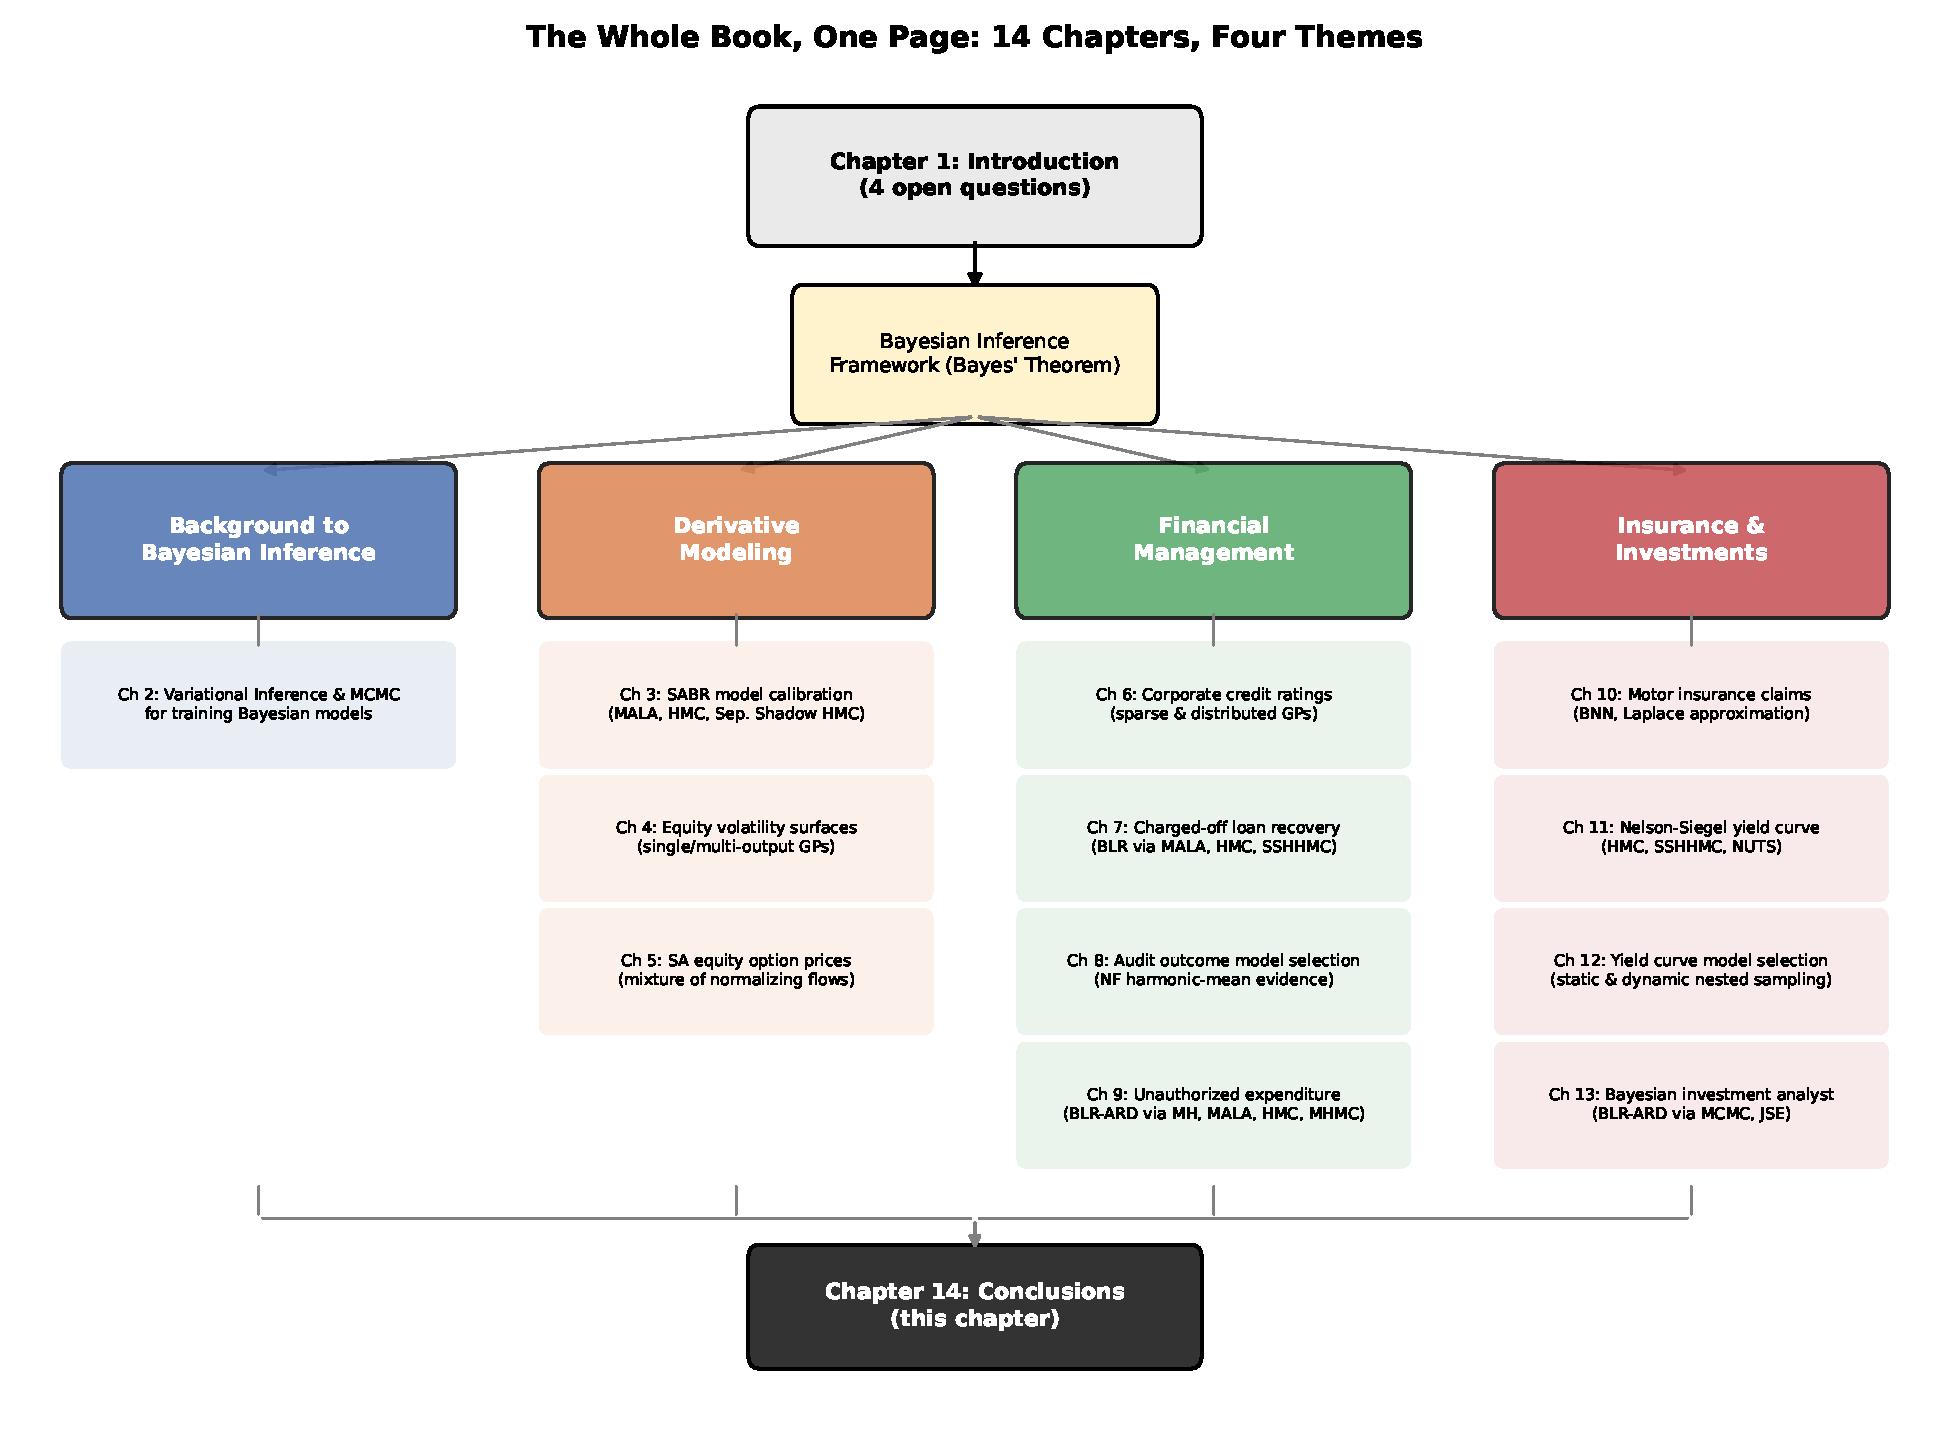
\includegraphics[width=0.92\textwidth]{fig_ch14_book_map.pdf}
  \end{center}
  \small The book's four themes (background, derivative modeling,
  financial management, insurance \& investments) sit on top of the same
  Bayesian inference core introduced in Chapter 1, and every theme feeds
  back into this concluding chapter.

\end{frame}

\begin{frame}{The Bayesian ML Toolkit, Chapter by Chapter}
  \begin{block}{Intuition}
    Across 11 application chapters, the book only ever reached for a
    handful of computational tools. Recognizing \emph{which} tool fits
    \emph{which} problem shape is one of the most transferable skills from
    this book.
  \end{block}
  \centering
  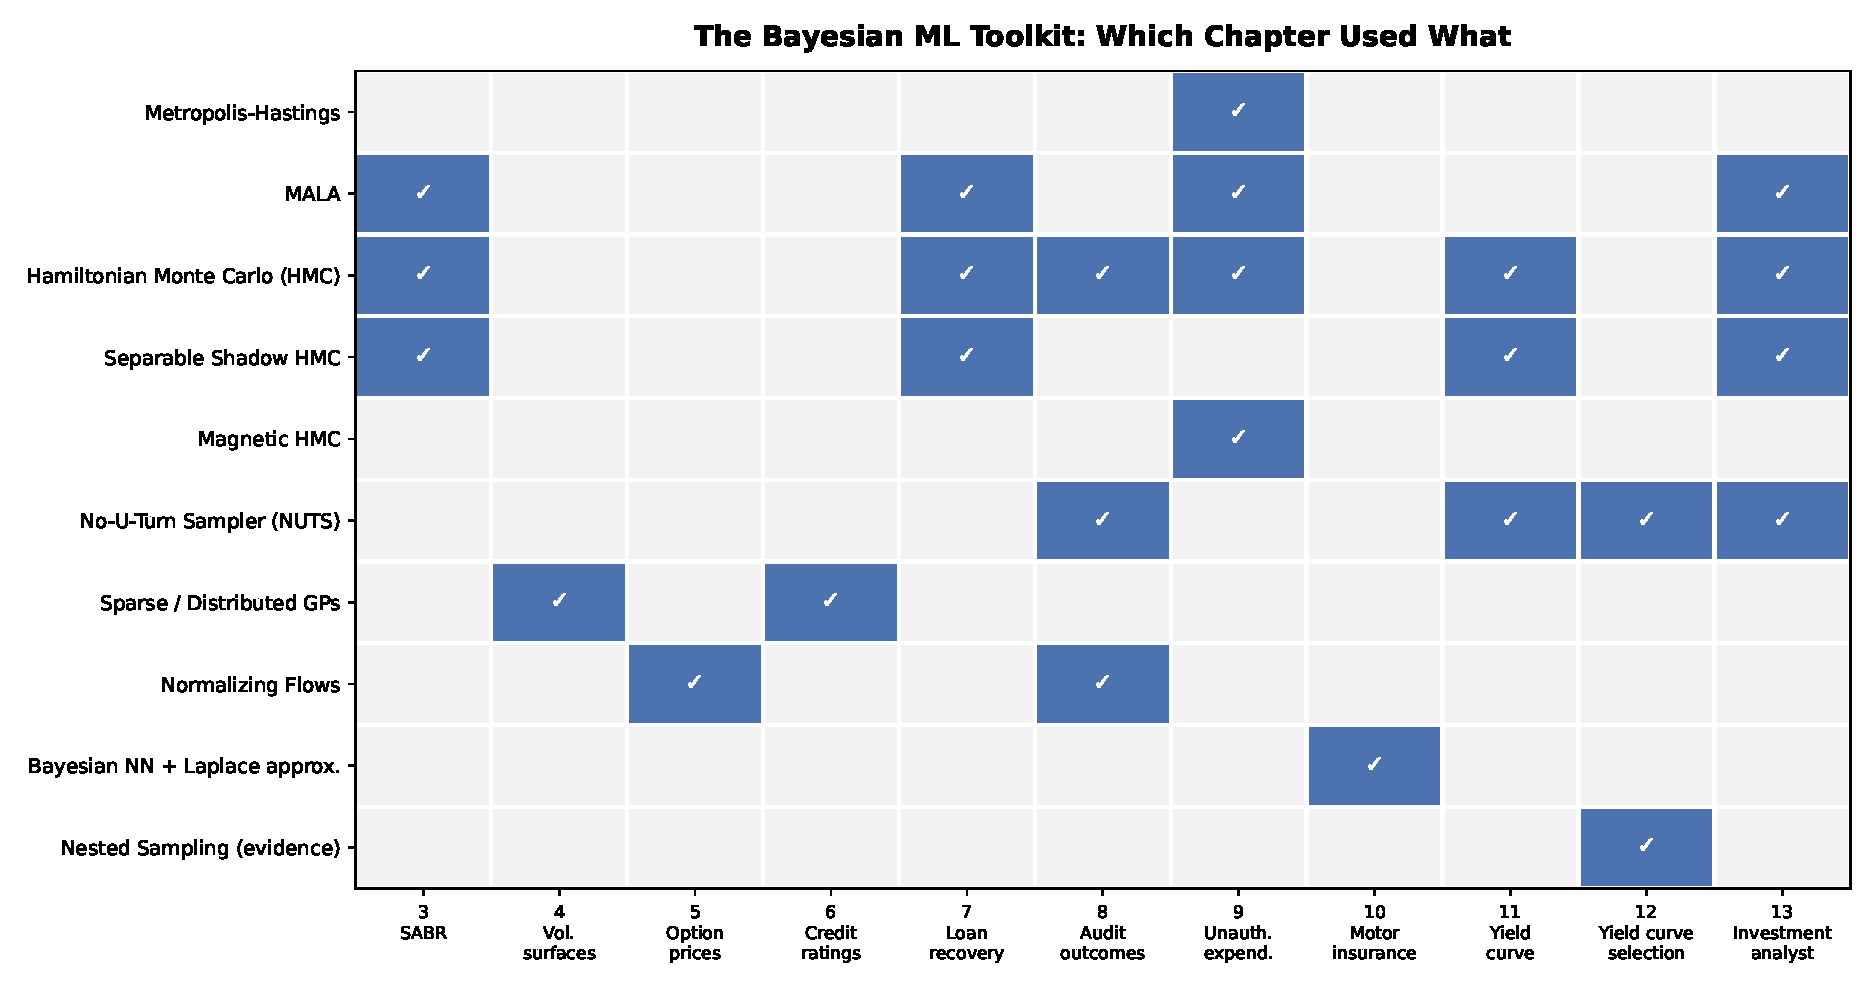
\includegraphics[width=0.92\textwidth]{fig_ch14_toolkit.pdf}

  \small Remember: MCMC variants (Chapters 3, 7--9, 11, 13) sample the
  posterior directly; GPs (Chapters 4, 6) place a distribution over a
  whole function; normalizing flows (Chapters 5, 8) build flexible
  learned densities; the BNN + Laplace approximation (Chapter 10) puts a
  distribution over network weights; nested sampling (Chapter 12) targets
  the evidence itself for model comparison.
\end{frame}

% ============================================================
\section{14.1 Summary of Contributions}
% ============================================================

\begin{frame}{14.1 Summary of Contributions: The Book's Own Framing}
  \begin{block}{What this book set out to do (in the authors' own words)}
    The advent of artificial intelligence and data-driven methods is
    transforming quantitative finance. This book explored various domains
    in quantitative finance and presented the theory and case studies of
    the potential of machine learning in this space. Employing the
    Bayesian inference framework -- and consequently Bayesian machine
    learning -- lets us naturally answer:
    \begin{enumerate}
      \item How can we \textbf{explain} the prediction or output of a model?
      \item What is the \textbf{distribution} of the model's parameters?
      \item How do we \textbf{select between} different models in a
      statistically principled manner?
      \item Which \textbf{inputs} are most relevant for the task at hand?
    \end{enumerate}
  \end{block}
  \textbf{Remember Chapter 1?} These are exactly the four open questions
  that motivated the whole book. The framework was applied across
  \emph{derivative modeling}, \emph{banking}, \emph{financial
  management}, \emph{insurance}, and \emph{investments} domains.
\end{frame}

\begin{frame}{Theme 0 -- Background to Bayesian Inference}
  \begin{block}{What the book says}
    For this theme, we explored the Bayesian paradigm and how this
    translates to Bayesian machine learning. We discussed the advantages
    and disadvantages of the Bayesian framework, how Bayesian models can
    be trained and deployed, and the performance metrics used to assess
    them. We further explored how the framework applies across derivative
    modeling, banking, financial management, insurance, and investments,
    and highlighted the impact machine learning is having on the finance
    industry.
  \end{block}
  \textbf{Remember Chapter 2?} This is precisely where MALA, HMC, NUTS,
  Separable Shadow HMC, and Magnetic HMC were introduced as the workhorse
  samplers that every later application chapter reused.
\end{frame}

\begin{frame}[allowframebreaks]{Theme 1 -- Derivative Modeling: Contributions}
  \begin{block}{SABR model calibration (Chapter 3)}
    We calibrated the Stochastic Alpha Beta Rho model with MALA, HMC, and
    Separable Shadow Hamiltonian Hybrid Monte Carlo. The approach
    precisely prices the interest-rate volatility skew on both simulated
    and ZAR swaption data, with the added benefit of a
    \emph{distribution} over model predictions and parameters. The MCMC
    methods are reasonably confident around the at-the-money point but
    less confident deep in/out of the money, and more confident on the
    skew's right wing than its left wing -- useful for generating
    volatility stress scenarios.
  \end{block}
  \begin{block}{Equity volatility surfaces (Chapter 4)}
    Single- and multi-output Gaussian processes, applied to equity
    volatility surface data from emerging (South Africa) and developed
    (Europe) markets, calibrate the rough Bergomi and Heston stochastic
    volatility models. Accuracy is similar to deep neural networks, with
    the added benefit of uncertainty across the surface and fewer
    hyperparameter configurations. Calibration becomes more specific
    (narrower confidence bands) at shorter maturities and at lower
    relative moneyness.
  \end{block}

  \framebreak

  \begin{block}{Option prices via normalizing flows (Chapter 5)}
    We priced European equity options in an emerging-market context with
    an entirely data-driven approach based on normalizing flows --
    learning the risk-neutral density directly (which already imposes
    no-arbitrage conditions) rather than bolting external arbitrage
    constraints onto the loss function. A mixture of normalizing flows
    reproduces option prices across maturities and moneyness levels;
    options close to expiry require more mixture components, and the
    largest pricing errors occur at low strikes.
  \end{block}

  \textbf{Remember Chapters 3--5?} Three different tools (MCMC, GPs,
  normalizing flows), one shared payoff: every derivative-modeling result
  in this book comes with a distribution, not just a point price.

  \centering
  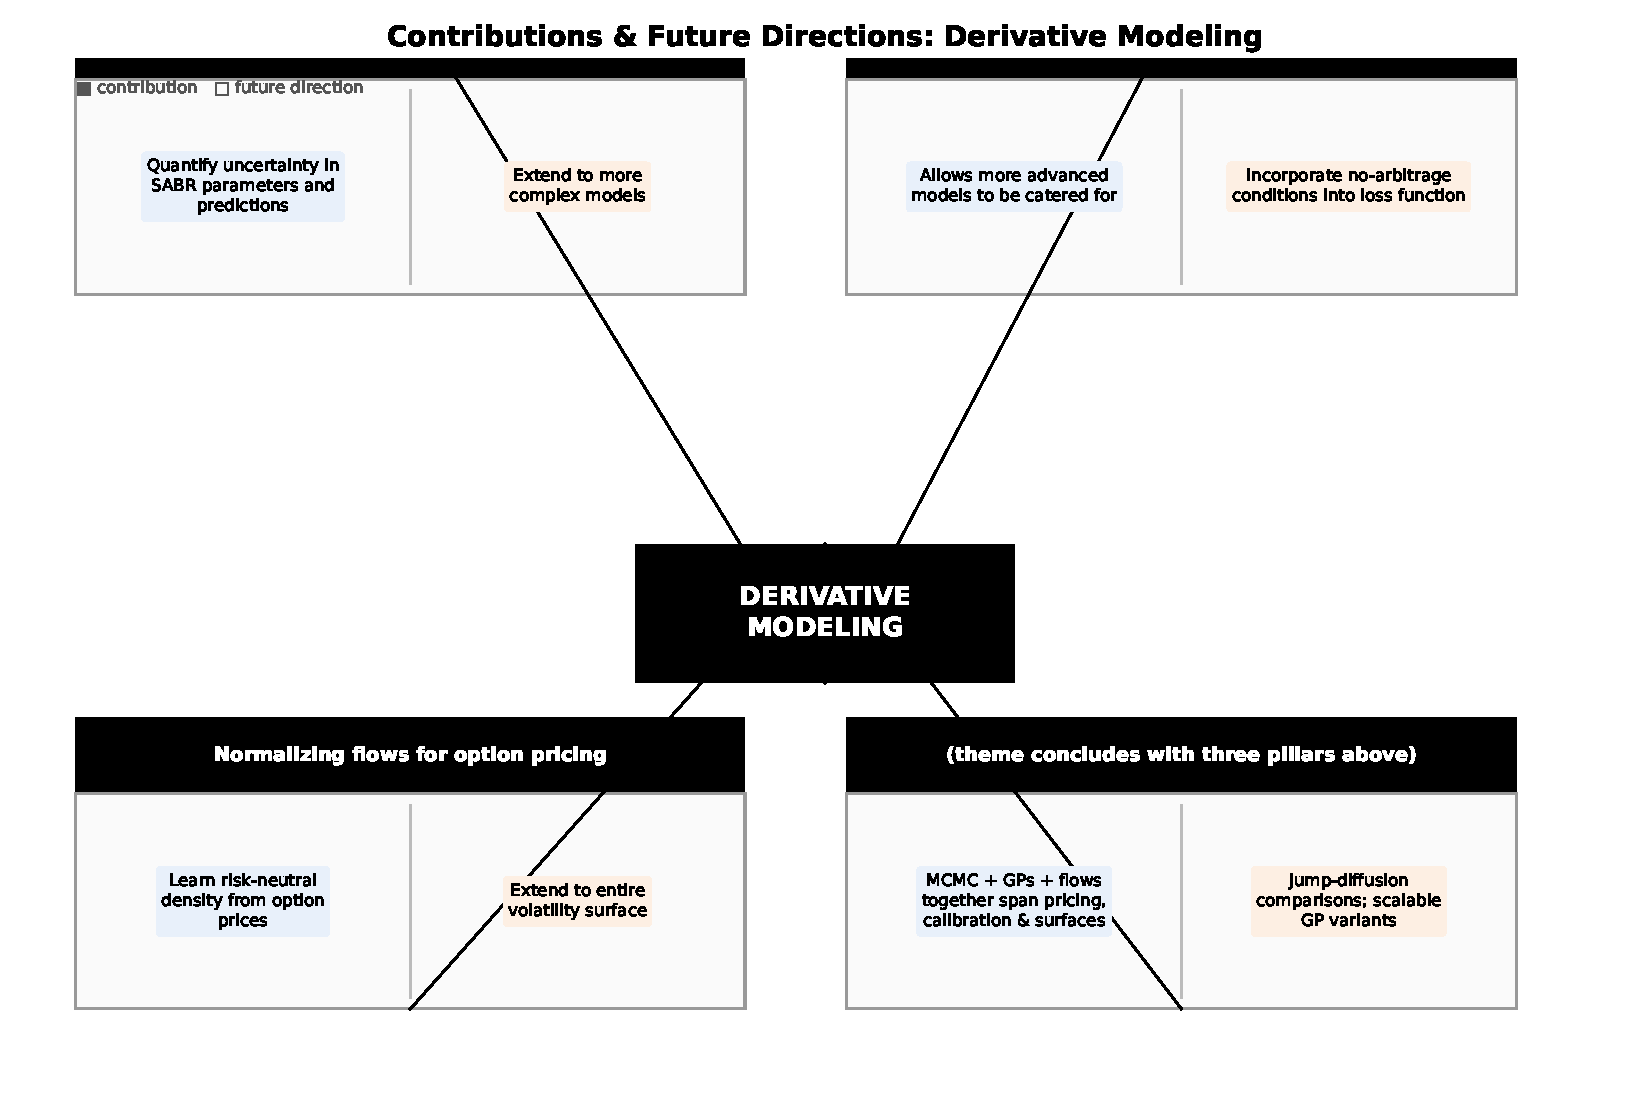
\includegraphics[width=0.82\textwidth]{fig_ch14_derivative_modeling.pdf}
\end{frame}

\begin{frame}[allowframebreaks]{Theme 2 -- Financial Management: Contributions}
  \begin{block}{Corporate credit ratings (Chapter 6)}
    Sparse and distributed Gaussian processes -- variations of the
    product-of-experts distributed GP -- predict corporate credit
    ratings and scale favorably to large datasets compared with classical
    GPs. The \emph{debt ratio}, \emph{profit margin-related} metrics, and
    \emph{return on capital ratio} are the most important financial
    metrics driving corporate credit rating.
  \end{block}
  \begin{block}{Recovery on charged-off loans (Chapter 7)}
    A Bayesian logistic regression model, trained with MALA, HMC, and
    Separable Shadow HMC, detects whether recoveries occur on
    non-performing loans. The \emph{purpose} of the loan,
    \emph{home-ownership} status, and the \emph{interest rate} charged
    are key features. The framework can be extended to more complex
    models such as Bayesian deep neural networks.
  \end{block}

  \framebreak

  \begin{block}{Audit outcome model selection (Chapter 8)}
    For municipal audit opinions, we compared Bayesian logistic
    regression models with varying numbers of covariates using the
    \textbf{Bayesian evidence}, estimated via a harmonic-mean estimator
    whose target distribution is learned with normalizing flows (fed by
    MALA/HMC/NUTS samples). The evidence computed on training data
    reliably predicts which model will outperform on unseen data, with a
    positive correlation to the Area Under the ROC Curve.
  \end{block}
  \begin{block}{Unauthorized expenditure (Chapter 9)}
    A Bayesian logistic regression model with an \textbf{automatic
    relevance determination (BLR-ARD)} prior, trained with
    Metropolis-Hastings, MALA, HMC, and Magnetic HMC, automatically ranks
    the input features most relevant to detecting unauthorized
    expenditure in South African municipalities -- a tool auditors can
    use for risk-rating municipal accounts, extendable to irregular and
    wasteful expenditure.
  \end{block}

  \textbf{Remember Chapters 6--9?} The evidence metric from Chapter 2's
  toolbox reappears here as the statistically principled way to
  \emph{select} between models -- the third of the book's four open
  questions, answered concretely.

  \centering
  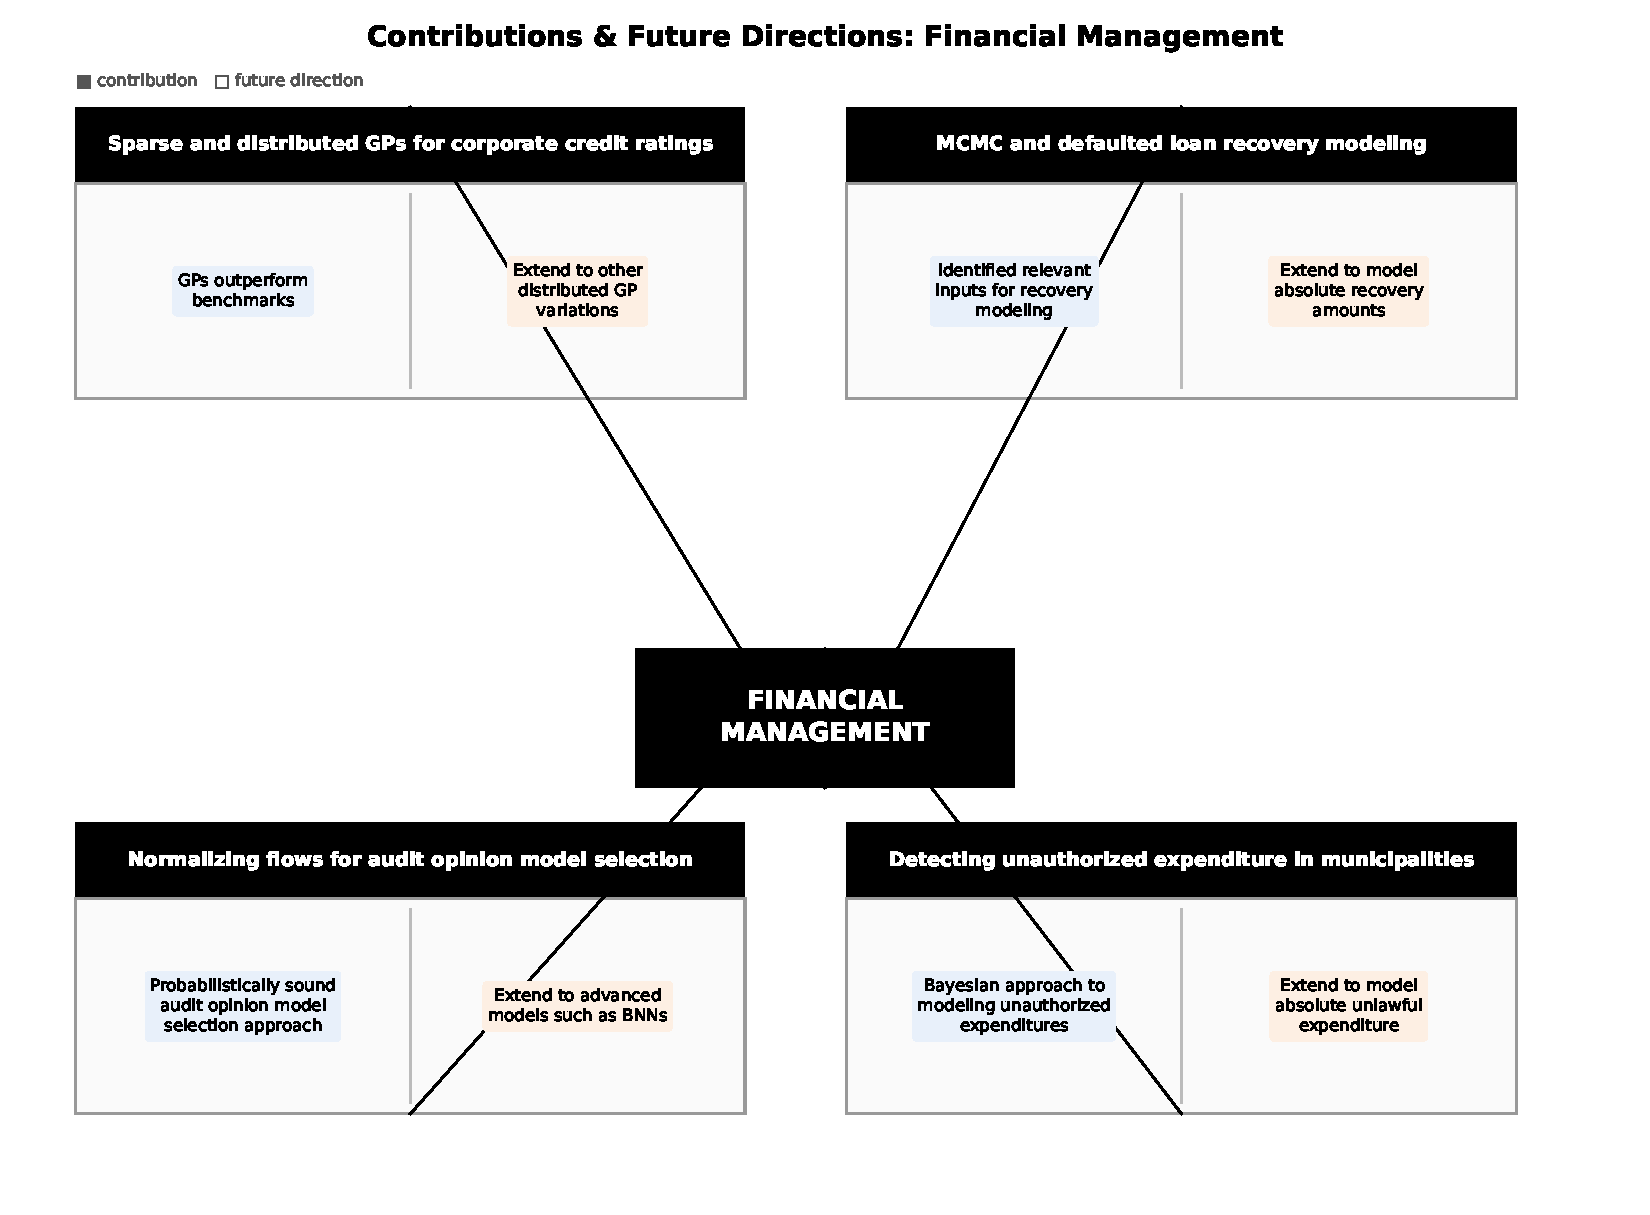
\includegraphics[width=0.82\textwidth]{fig_ch14_financial_management.pdf}
\end{frame}

\begin{frame}[allowframebreaks]{Theme 3 -- Insurance and Investments: Contributions}
  \begin{block}{Motor insurance claims (Chapter 10)}
    We modeled the likelihood of motor insurance claims using Bayesian
    neural networks trained with the Laplace (Gaussian) approximation of
    MacKay (1992) -- a variational inference variant. Deeper
    architectures outperform wider ones, and the Bayesian evidence
    selects the architecture that generalizes best. An ARD prior
    identifies \emph{claims history}, \emph{type of fuel}, \emph{power of
    the vehicle}, \emph{lapse}, and \emph{number of policies} as the
    essential features -- making an otherwise black-box neural network
    interpretable to non-expert stakeholders.
  \end{block}
  \begin{block}{Nelson--Siegel yield curve calibration (Chapter 11)}
    We calibrated the Nelson \& Siegel (1987) yield curve model with HMC,
    Separable Shadow Hybrid HMC, and NUTS. The calibration gives
    comparable or better yield curve estimates than ordinary least
    squares across multiple performance metrics, with a full account of
    parameter uncertainty.
  \end{block}

  \framebreak

  \begin{block}{Yield curve model selection (Chapter 12)}
    We used the \textbf{nested sampling} evidence estimation method of
    Skilling (2004) to select between nested Nelson--Siegel models, and
    introduced the \textbf{ARD-Nelson-Siegel (ARD-NS)} model, trained
    with NUTS, which automatically ranks the short-, medium-, and
    long-term factor loadings. The evidence framework reliably detects
    the model that generated the data, and the ARD-NS model shows that
    yield curve dynamics are driven mainly by the \emph{medium-term
    (curvature)} factor loading.
  \end{block}
  \begin{block}{Bayesian investment analyst (Chapter 13)}
    A BLR-ARD model trained with MCMC methods builds a Bayesian
    sell-side investment analyst for JSE-listed stocks. It has the best
    performance on industrial stocks, then resources, then financial
    stocks, and outperforms the mean consensus of sell-side analysts
    across all four experiments considered. \emph{Relative volatility}
    and \emph{initial price} matter most for the full JSE universe; the
    important features vary meaningfully by sector.
  \end{block}

  \textbf{Remember Chapters 10--13?} BNNs (Chapter 10) and nested
  sampling (Chapter 12) are the two tools we had not yet used elsewhere
  in the book -- both introduced precisely because insurance claims and
  yield curve model selection needed them.

  \centering
  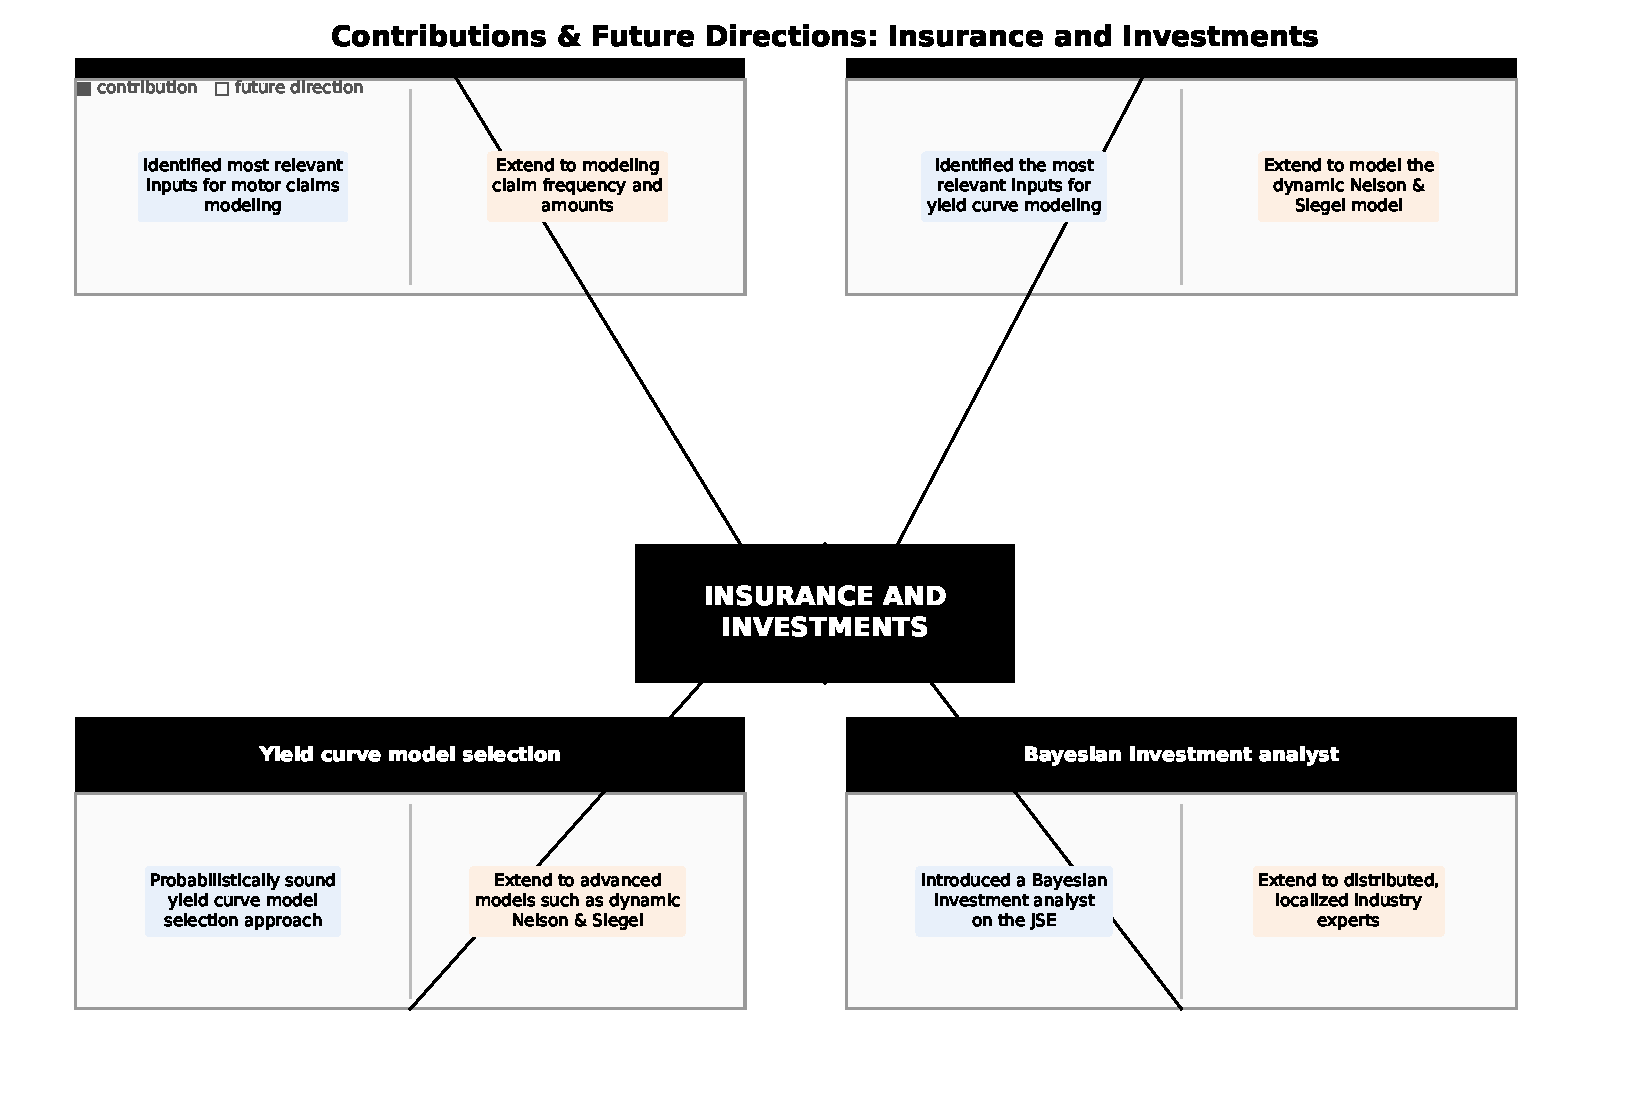
\includegraphics[width=0.82\textwidth]{fig_ch14_insurance_investments.pdf}

  \small \emph{A close read of the book's own Fig.\ 14.3:} its
  Nelson--Siegel panel text is worded almost identically to the loan
  recovery panel in Fig.\ 14.2 -- an artifact in the original figure. The
  running text of Section 14.1 (reproduced above) is unambiguous about
  what was actually contributed, and that is what is summarized here.
\end{frame}

% ============================================================
\section{14.2 Ongoing and Future Research Directions}
% ============================================================

\begin{frame}{14.2 Ongoing and Future Research Directions}
  \begin{block}{Setting the scene (in the authors' own words)}
    This book has highlighted various problems in quantitative finance
    where the Bayesian framework produced good insights. However, many
    domains within quantitative finance -- and other models and
    algorithms -- still need to be explored to extend the work presented
    in this manuscript. A summary of ongoing and future research across
    the themes covered in this book follows.
  \end{block}
  \textbf{Why this matters for you:} every future direction below is a
  natural ``next chapter'' you could now write yourself, using tools
  already in your hands from Chapters 2--13.
\end{frame}

\begin{frame}[allowframebreaks]{Future Directions -- Derivative Modeling}
  \begin{block}{SABR calibration (extends Chapter 3)}
    Enhance by considering the \emph{entire} interest-rate volatility
    surface, rather than limiting data to the 1W-into-1Y and 6M-into-1Y
    swaptions used in this book. Compare against other models that
    capture the volatility skew, such as jump-diffusion models (Mongwe,
    2015; Mongwe et al., 2022).
  \end{block}
  \begin{block}{Volatility surface GPs (extends Chapter 4)}
    Improve by ensuring the inducing points and kernels used for the
    multi-output GP are \emph{not} shared. All models in this book
    approximated the pricing function without explicitly incorporating
    no-arbitrage conditions (Sidogi et al., 2022) -- future work will
    incorporate them explicitly. A key limitation is the computational
    complexity of GPs; state-of-the-art scaling approaches, such as
    distributional GPs (Cohen et al., 2020), are a planned remedy.
  \end{block}

  \framebreak

  \begin{block}{Normalizing flows for option pricing (extends Chapter 5)}
    Compare various techniques for \emph{optimally selecting the number
    of mixture components} in the normalizing flow mixture. It could
    also be interesting to jointly model the \emph{entire} option price
    surface (across all expiries and strikes) instead of the volatility
    skew per expiry (Yang \& Hospedales, 2023).
  \end{block}
  \textbf{Remember Chapter 4's discussion of no-arbitrage conditions?}
  This is precisely the limitation future work aims to close, on both
  the GP and normalizing-flow sides of the derivative modeling theme.
\end{frame}

\begin{frame}[allowframebreaks]{Future Directions -- Financial Management}
  \begin{block}{Credit ratings via distributed GPs (extends Chapter 6)}
    Expand by considering other distributed GPs, such as a
    \emph{mixture} of experts instead of a \emph{product} of experts.
    Data from a developing nation such as South Africa could also assess
    model performance, and selecting the \emph{number of experts} for the
    distributed GP is itself an open problem (Cohen et al., 2020).
  \end{block}
  \begin{block}{Loan recovery modeling (extends Chapter 7)}
    Extend to more complex models such as deep neural networks. Rather
    than only detecting \emph{whether} recoveries are present, modeling
    the \emph{actual absolute recovery amount} on the defaulted loan
    using Bayesian techniques is an open problem, still unexplored in
    detail in the literature.
  \end{block}

  \framebreak

  \begin{block}{Audit opinion model selection (extends Chapter 8)}
    Extend to more complicated models, such as deep neural networks, and
    more advanced sampling techniques based on Riemannian manifolds
    (Marwala et al., 2023; Mongwe et al., 2021b). Compare the model
    selection results against other Bayesian evidence estimation
    approaches, such as nested sampling (Skilling, 2004; Speagle, 2020).
  \end{block}
  \begin{block}{Unauthorized expenditure (extends Chapter 9)}
    Expand to model the \emph{absolute value} of unauthorized
    expenditure, and jointly model other unlawful spending such as
    \emph{fruitless and wasteful expenditure}. Explore more complex
    models, such as Bayesian neural networks, for this task.
  \end{block}

  \textbf{Remember Chapter 12's nested sampling?} Notice it resurfaces
  here as a proposed \emph{alternative} evidence-estimation method for
  the audit-opinion model-selection problem of Chapter 8 -- the book's
  own future work cross-pollinates between its themes.
\end{frame}

\begin{frame}[allowframebreaks]{Future Directions -- Insurance and Investments}
  \begin{block}{Motor insurance claims (extends Chapter 10)}
    Scale the Bayesian neural network to larger models and select
    between different models/architectures. Consider other BNN training
    methods, such as MCMC, that guarantee convergence to the true target
    posterior. Instead of only forecasting \emph{whether} a claim occurs,
    extend to model the \emph{absolute value} of claims through analysis
    of claim frequency and severity.
  \end{block}
  \begin{block}{Nelson--Siegel yield curve (extends Chapters 11--12)}
    Extend the analysis to the \textbf{dynamic Nelson-Siegel model},
    which captures yield curve dynamics over time, and to modeling the
    \emph{term structure of volatilities} using the Nelson-Siegel model
    (promising initial results in Guo et al., 2014). For model selection,
    incorporate yield curve models beyond variations/subsets of
    Nelson-Siegel, and try other evidence-calculation methods, such as
    normalizing flows and the harmonic mean estimator (Polanska et al.,
    2023).
  \end{block}

  \framebreak

  \begin{block}{Bayesian investment analyst (extends Chapter 13)}
    Consider more complicated models, such as Bayesian neural networks,
    instead of Bayesian logistic regression (Mbuvha et al., 2021).
    Training \emph{experts in each sector} and aggregating results could
    significantly improve performance -- potentially approached with
    distributed GP models such as the product-of-experts (Cohen et al.,
    2020).
  \end{block}
  \begin{block}{Other themes not covered in this book}
    Machine learning has also been used for: hedging options (deep
    hedging, Buehler et al., 2019), predicting stock prices from limit
    order book data (Sidogi et al., 2023), and generating synthetic
    financial markets data (Sidogi et al., 2022). These and other
    problems are ripe for framing within the Bayesian framework.
  \end{block}

  \textbf{Remember Chapter 6's product-of-experts GP?} It is proposed
  again here, in Chapter 13's future work, as a way to build
  \emph{distributed, localized industry experts} for the investment
  analyst -- the same tool, a new application.
\end{frame}

\begin{frame}{Closing Words of the Book}
  \begin{block}{In the authors' own words}
    As highlighted above and throughout this book, there are various
    avenues that one can explore to enhance and extend the work presented
    across the different themes in this book. We look forward to the
    increased deployment of Bayesian inference frameworks in practice
    within the quantitative finance domain.
  \end{block}
  \textbf{Remember the coin flip from Chapter 1?} Every idea in this
  book -- SABR skews, credit ratings, audit opinions, motor claims,
  yield curves, JSE stock calls -- was that same coin-flip logic, applied
  at scale: start with a belief, observe data, update the belief, and
  keep the resulting \emph{uncertainty} rather than throwing it away.
\end{frame}

% ============================================================
\section{Key Takeaways}
% ============================================================

\begin{frame}[allowframebreaks]{Key Takeaways: One Idea per Method Family}
  \begin{itemize}
    \item \textbf{Bayesian thinking (Ch.\ 1--2):} treat unknowns as
    distributions, not single numbers -- the posterior
    $\Prob(\thetav\mid\Data)\propto \Prob(\Data\mid\thetav)\Prob(\thetav)$
    is the object of interest, always.
    \item \textbf{MCMC / HMC family (MALA, HMC, Separable Shadow HMC,
    Magnetic HMC, NUTS -- Ch.\ 3, 7--9, 11, 13):} when there is no
    closed-form posterior, simulate samples from it; gradient information
    (Hamiltonian dynamics) makes sampling efficient in high dimensions.
    \item \textbf{Gaussian processes (Ch.\ 4, 6):} put a Bayesian belief
    over an entire \emph{function} (a volatility surface, a rating
    function), and use sparsity/distribution tricks to make that
    tractable at scale.
    \item \textbf{Normalizing flows (Ch.\ 5, 8):} learn flexible,
    invertible probability distributions directly from data -- useful
    both for pricing (learning a risk-neutral density) and for
    estimating hard normalizing constants (the evidence).

    \framebreak

    \item \textbf{Bayesian neural networks (Ch.\ 10):} a distribution
    over network weights turns a black box into an
    uncertainty-aware, and via ARD, an \emph{interpretable} predictor.
    \item \textbf{Nested sampling / the evidence (Ch.\ 8, 12):} the
    evidence $\Prob(\Data)=\int \Prob(\Data\mid\thetav)\Prob(\thetav)\,d\thetav$
    is not just a normalizing constant -- it is a principled,
    automatic way to compare and select between competing models.
    \item \textbf{Automatic relevance determination (Ch.\ 6, 9, 10, 12,
    13):} a prior can do double duty as a feature-selection mechanism,
    ranking which inputs actually drive the prediction.
    \item \textbf{The unifying thread:} every application in this book
    answers the same four questions from Chapter 1 -- explainability,
    parameter uncertainty, principled model selection, and input
    relevance -- by staying faithful to one formula, applied
    imaginatively across derivative pricing, credit, audit, insurance,
    and investment problems.
  \end{itemize}
\end{frame}

\end{document}
